\chapter{System Design and Methodology}

This chapter details the proposed architecture and implementation strategy of the agentic AI framework designed to support multi-cloud architectural decision-making. It outlines the constructive research methodology, system domain specifics, agentic architecture, key algorithms, and the tools and technologies employed.

\section{Research Design}

The research methodology follows a constructive research approach, also known as design science, where a novel artifact is systematically designed, implemented, and empirically evaluated to address a practical problem—in this case, cloud architecture recommendation and validation. This approach emphasizes iterative cycles of design, software development, and quantitative/qualitative assessment. In the context of this thesis, the constructive artifact is the Agentic AI Framework, and the empirical evaluation is conducted using the quantitative NLP metrics detailed in Chapter 5.

\section{System Domain: Amazon Web Services (AWS)}

The initial focus domain is Amazon Web Services (AWS), the leading public cloud provider offering hundreds of interrelated services. Many services share overlapping functionalities but differ in tradeoffs (e.g., Amazon ECS, EKS, and Lambda for compute workloads). Such complexity necessitates automated decision-support tools.

Within the framework, agents specialize across four core AWS service domains:

\begin{itemize}
    \item \textbf{Compute:} Handling services such as EC2, ECS, Lambda, etc.
    \item \textbf{Network:} Managing VPCs, subnets, gateways, security groups, etc.
    \item \textbf{Storage:} Covering S3, EBS, EFS, Glacier, etc.
    \item \textbf{Database:} Including RDS, DynamoDB, and related analytics services.
\end{itemize}

This domain decomposition leverages architect expertise modularly within the multi-agent architecture.

\section{System Architecture}

The proposed system is an autonomous multi-agent framework designed to emulate a collaborative team of expert solution architects. It is realized as a cyclic state machine graph orchestrated via LangGraph \cite{langgraph2024docs} enabling iterative workflows.

\begin{figure}[h]
  \begin{center}
  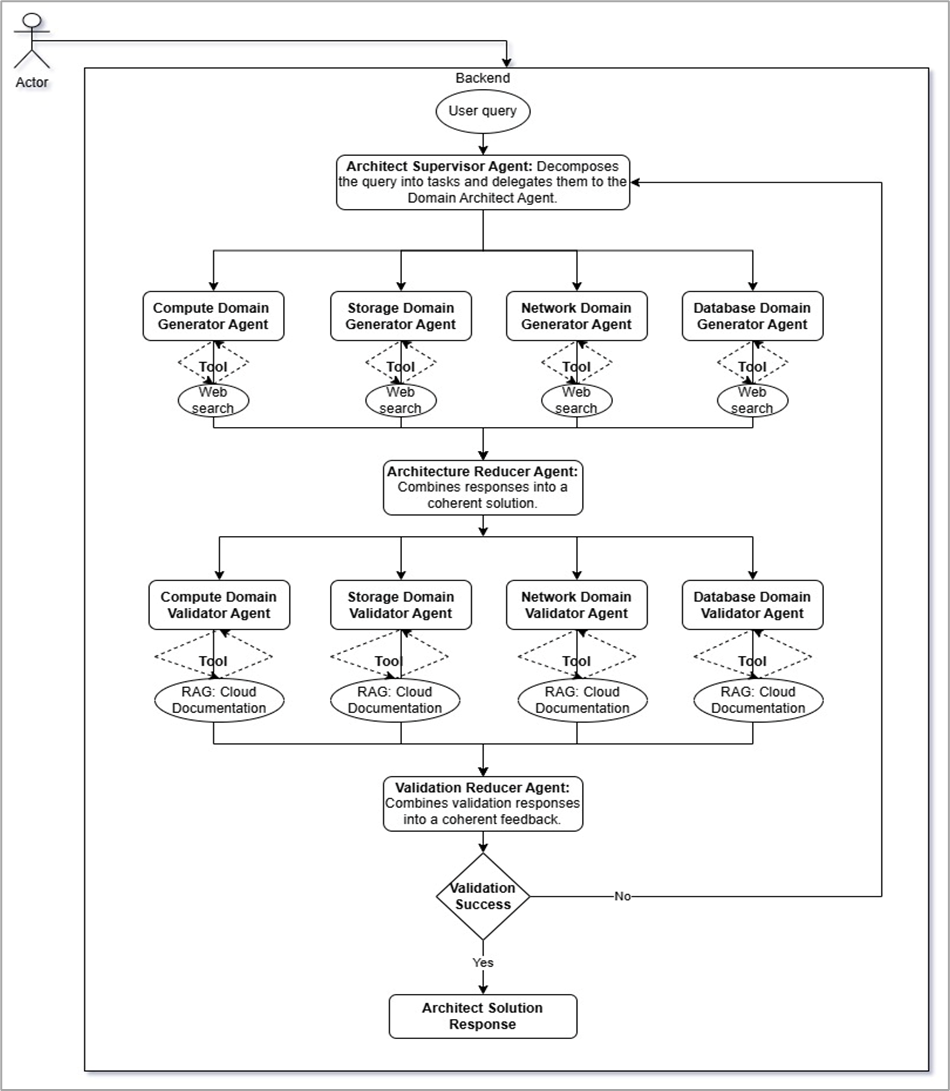
\includegraphics[width=11cm, height=12cm]{AgenticArchitect.png}
  \caption{Agent Framework: System Architecture Design}
  \label{fig:system_arch}
  \end{center}
\end{figure}

The architecture operates in five distinct phases managed by a graph-based state machine:

\subsection{Phase 1: Query Decomposition}

An external actor submits a natural language \textbf{User Query} describing desired cloud architecture requirements. The \textbf{Architect Supervisor Agent} parses and decomposes this query into discrete domain-specific tasks, distributing responsibilities across specialized agents to maximize parallelism and expertise application.

\subsection{Phase 2: Generation (Drafting the Solution)}

\textbf{Generator Agents} operate in parallel within their specialized domains (compute, network, storage, database), leveraging a ReAct-based interaction style \cite{yao2023react} combined with a \textbf{Web Search} tool (using Google Serper API) to inform solution drafting with the latest cloud service information and best practices.

\subsection{Phase 3: Synthesis}

An \textbf{Architecture Reducer Agent} aggregates and synthesizes the discrete partial solutions generated by domain-specific agents into a coherent, integrated cloud architecture proposal.

\subsection{Phase 4: Validation (Checking the Work)}

Parallel \textbf{Validator Agents} evaluate the synthesized draft architecture against official, vendor-provided documentation as accessed via a Retrieval-Augmented Generation (RAG) tool \cite{lewis2020rag} grounded in a vector database leveraging \texttt{ChromaDB} for fast, semantic similarity searches of embedded AWS documentation processed and stored.

\subsection{Phase 5: Iteration and Response}

A \textbf{Validation Reducer Agent} consolidates validator feedback, assessing evaluation outcomes. If validation metrics or expert judgement criteria are not met, feedback is escalated to the Supervisor Agent to restart query decomposition and solution refinement. Upon successful validation, a final \textbf{Architect Solution Response} is generated and delivered to the end-user.

\section{Algorithms and Techniques}

\subsection{Core Workflow: Evaluator-Optimizer}

The central workflow is a self-correcting "Evaluator-Optimizer" loop depicted in Figure \ref{fig:eval_workflow}, inspired by \cite{anthropic2024agents}. In each iteration, a Generator Agent proposes an architectural solution, which a Validator Agent critiques using RAG grounded in up-to-date vector database retrievals. This cycle iterates until the solution passes validation thresholds, ensuring factual accuracy and compliance.

\begin{figure}[h]
    \centering
    \fbox{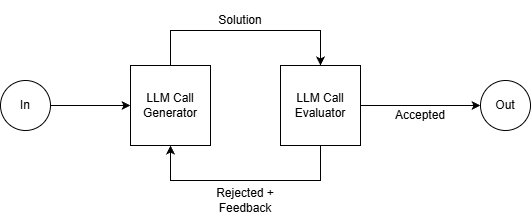
\includegraphics[width=0.9\textwidth]{Evalutor-Optimiser.drawio.png}}
    \caption[The Evaluator-Optimizer Workflow]{The Evaluator-Optimizer Workflow (Source: Adapted from \cite{anthropic2024agents})}
    \label{fig:eval_workflow}
\end{figure}

\subsection{Knowledge Base Construction (Data Pipeline)}

A robust knowledge base underpins RAG validation, constructed in four stages:

\begin{enumerate}
    \item \textbf{Data Collection:} Web scraping of official AWS documentation ensures the inclusion of comprehensive, up-to-date cloud service knowledge. The Beautiful Soup Python library is used for extraction. Both automated and manual scraping methods were implemented because AWS documentation often has inconsistent webpages, naming conventions, and structural formats. Some services provide a User Guide, others a Developer Guide, and overall the documentation structures vary significantly.
    \item \textbf{Data Preprocessing:} The \textbf{Docling} AI-driven parser \cite{docling2025paper}, \cite{docling2024web} processes complex PDF and DOCX whitepapers into uniform, clean text. The data is preprocessed by converting PDFs to Markdown and then removing elements such as images, irrelevant tables, and other non-vectorizable content. Metadata, such as service name and source URL is then added to facilitate efficient filtering.
    \item \textbf{Embedding Generation:} The \textbf{Ollama}-served \texttt{nomic-embed-text} model converts textual chunks into dense vector embeddings that capture semantic relationships. The embedding generation was performed locally on a Mac device, leveraging the MPS capabilities of the Apple Silicon M2 chip.
    \item \textbf{Vector Storage and Retrieval:} ChromaDB manages embedding storage, enabling efficient similarity-based retrieval required for RAG mechanisms \cite{chromadb2024}. The vector database is persistently stored on the hard disk, allowing it to be reused in future operations.
\end{enumerate}

\section{Tools and Technologies}

The project prototype employs the following primary technologies and frameworks:

\begin{itemize}
    \item \textbf{Programming Language:} Python 3.10+ provides flexibility and robust libraries for AI and web integration.
    \item \textbf{LLM Models:} OpenAI GPT-4o and GPT-4o-mini are leveraged for natural language understanding and generation, with \texttt{nomic-embed-text} powering semantic vector embeddings. GPT-4o is used for higher-level reasoning tasks and agents such as the supervisor and synthesizer, while GPT-4o-mini is used for more specialized tasks and agents, such as compute domain architecture generation, storage domain validation, etc.
    \item \textbf{Agentic Framework:} LangGraph \cite{langgraph2024docs} enables cyclic, stateful multi-agent orchestration beyond linear pipelines.
    \item \textbf{LLM Orchestration:} LangChain \cite{langchain2024docs} and its Expression Language LCEL \cite{langchain2024lcel} streamline prompt management, chaining, and tool integration.
    \item \textbf{Local Embedding Service:} Ollama \cite{ollama2024web} with \texttt{nomic-embed-text} manages local LLM and embedding model.
    \item \textbf{Vector Database:} ChromaDB \cite{chromadb2024} indexes and enables fast semantic retrieval of vector embeddings crucial for RAG.
    \item \textbf{Live Data Integration:} Google Serper API is integrated to provide Generator Agents with real-time access to the latest cloud service documentation.
    \item \textbf{Graph Observability:} LangSmith is utilized to trace and debug the complex, non-deterministic execution paths of the cyclic multi-agent workflow.
    \item \textbf{Hardware Acceleration:} Apple Metal Performance Shaders (MPS) framework \cite{apple2024mps} accelerates embedding generation on Apple Silicon.
\end{itemize}

